% In your document preamble: \usepackage{booktabs}, \usepackage{hyperref}, \usepackage{longtable}, \usepackage{caption}
\scriptsize
\setlength{\tabcolsep}{3pt}
\begin{longtable}{llllrr@{\hspace{0.8cm}}llllrr}
\captionsetup{labelformat=empty}
\caption{\textbf{SI Table S10. Data for CBP Domain Receptors}}
\label{tab:st10} \\
\toprule
apo\_pdb & holo\_pdb & apo\_bmrb & holo\_bmrb & F1 & MCC & apo\_pdb & holo\_pdb & apo\_bmrb & holo\_bmrb & F1 & MCC \\
\midrule
\endfirsthead
\caption[]{(continued)} \\
\toprule
apo\_pdb & holo\_pdb & apo\_bmrb & holo\_bmrb & F1 & MCC & apo\_pdb & holo\_pdb & apo\_bmrb & holo\_bmrb & F1 & MCC \\
\midrule
\endhead
\bottomrule
\endfoot
\bottomrule
\endlastfoot
\href{https://www.rcsb.org/structure/1U2N}{1U2N} & \href{https://www.rcsb.org/structure/1R8U}{1R8U} & \href{https://bmrb.io/data_library/summary/index.php?bmrbId=6268}{6268} & \href{https://bmrb.io/data_library/summary/index.php?bmrbId=5987}{5987} & 0.56 & 0.24 &  &  &  &  &  &  \\
\end{longtable}

\begin{figure}[htbp]
\centering
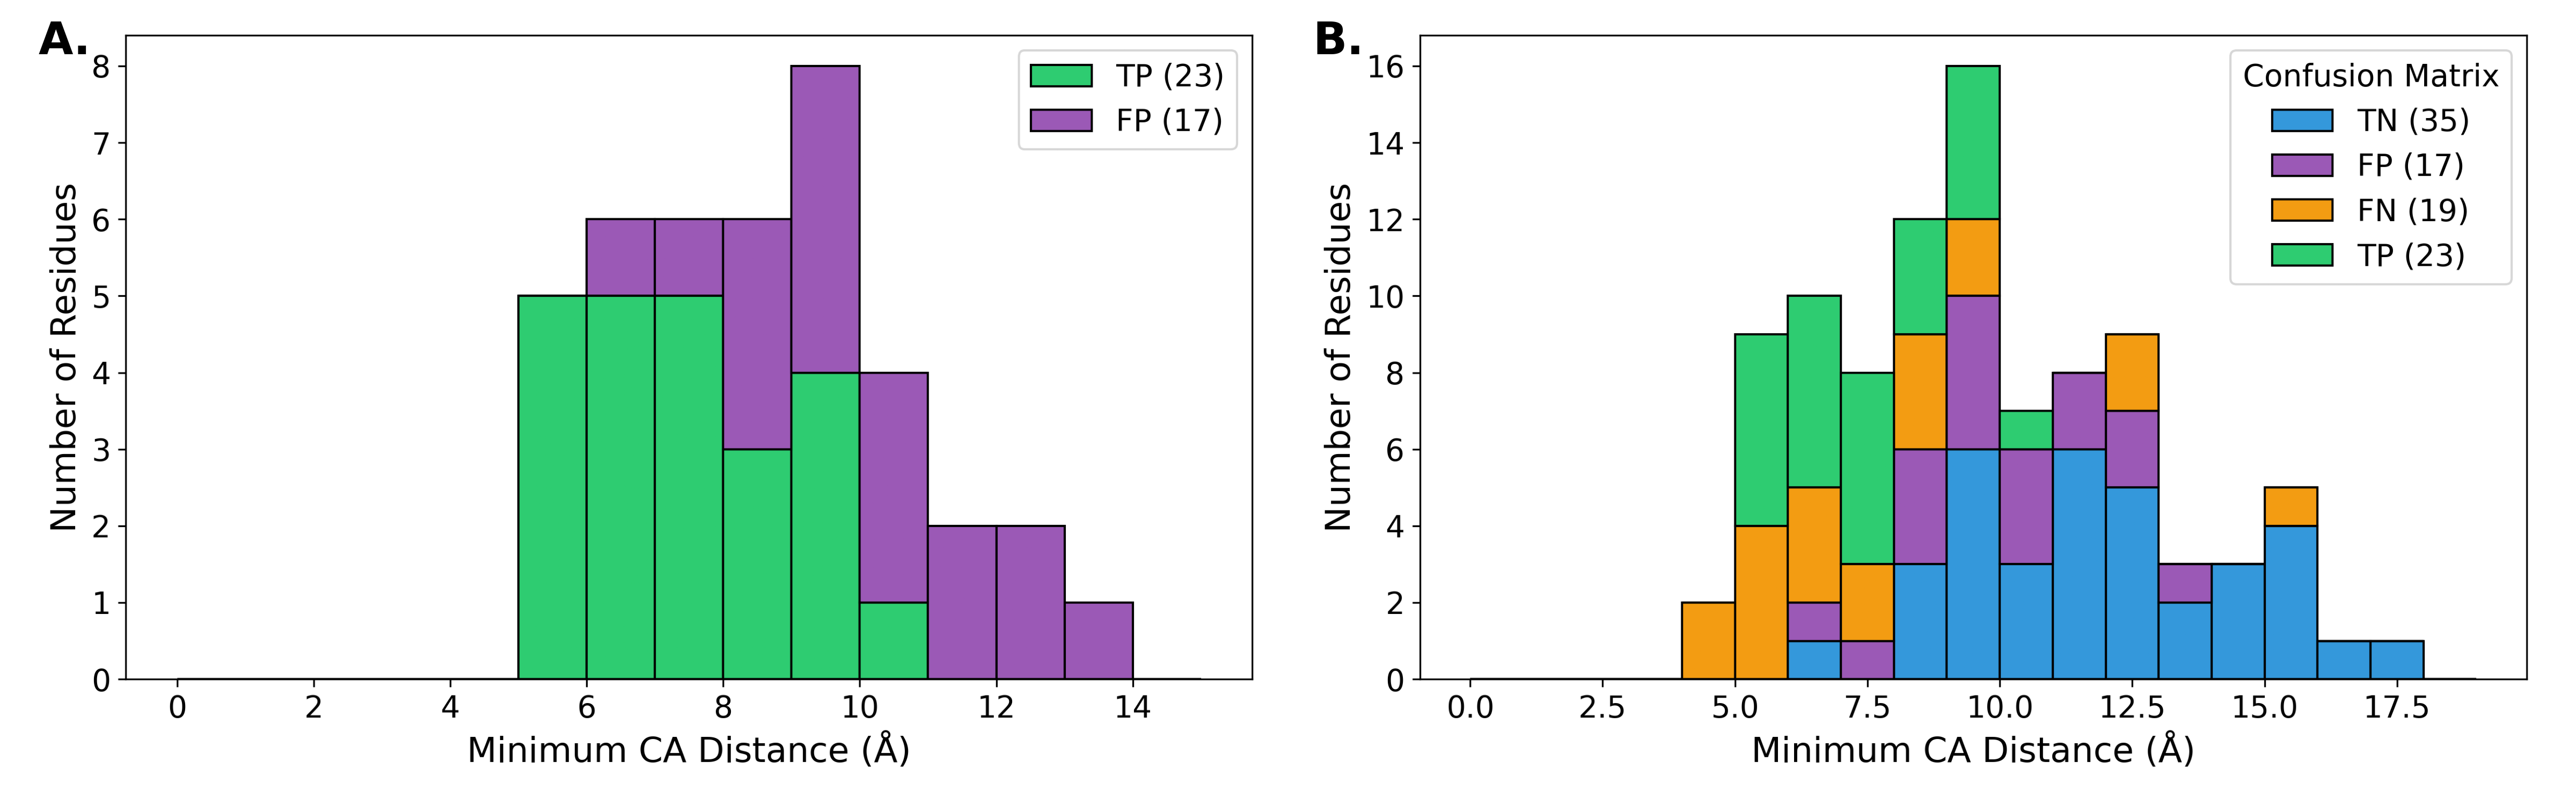
\includegraphics[width=\linewidth]{SF9_CBP.png}
\captionsetup{labelformat=empty}
\caption{\textbf{SI Fig. S9. Confusion Matrix Histograms for CBP Domain Receptors}}
\label{fig:sf9_cbp}
\end{figure}
